\subsection{Standardized Euclidean distance}
\label{section:SEuclidean}

\begin{figure}[t]
    \centering
    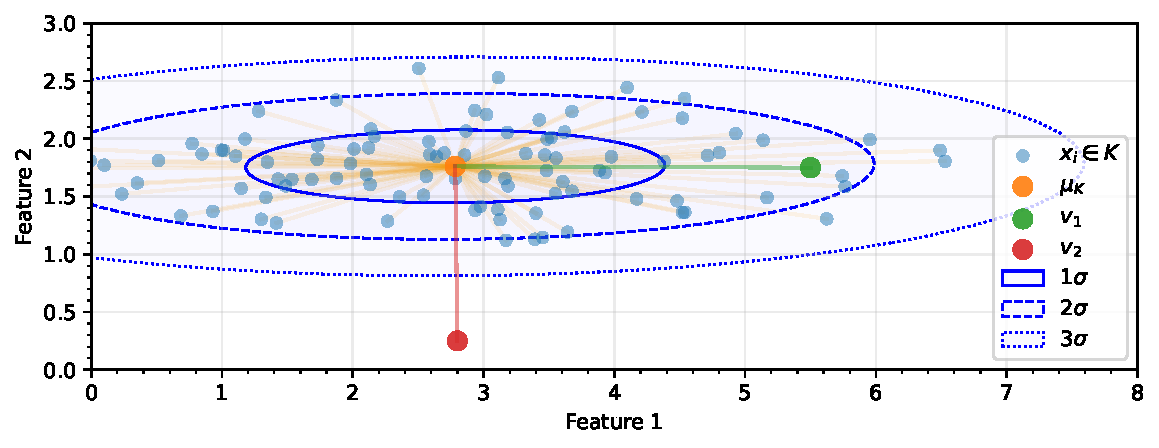
\includegraphics[width=\textwidth]{images/measures/seuclidean-distance.pdf}
    \caption{Idea of the Standardized Euclidean distance applied as an outlierness measure.
             Cluster $T$ displays the heterogeneous spread along the axes – higher variance
             on feature 1 and lower variance on feature 2. Considering the different variances,
             after scaling the axes ($\sigma_1 \approx 1.5$, $\sigma_2 \approx 0.3$),
             the element $v_1$ is located closer to center $\mu_K$ than the element $v_2$
             that is outlier (distance $d_1 \approx \frac{2.7}{1.5} \approx 1.8$,
             distance $d_2 \approx \frac{1.5}{0.3} \approx 5.0$).}
    \label{fig:sed-idea}
\end{figure}

The Standardized Euclidean distance is another measure based on Minkowski metric of order $2$ in $\mathbb{R}^d$ space – a square root of the sum of vector elements to the power of $2$. It considers axes-wise variances to normalize the contributions of each vectors elements when calculating the distance. It can be considered as a compromise between the traditional Euclidean distance, that assumes uniform relevance of all axes, and more general Mahalanobis distance, that estimates the distribution shape using the covariance matrix.

The outlierness score for a given vector $v$ against the data cluster $T$ is calculated as
\begin{equation}
    SED(v, T) = \sqrt{
        \sum_{j=1}^{d}
        \frac{1}{V_{T,j}}
        \cdot
        \left(
            v_{j} - \mu_{T,j}
        \right)^2
    }.
    \label{eq:sed}
\end{equation}

The $V_K$ represents a vector of variances; the $V_{T,j}$ is a variance along $j$-th axis in cluster $T$ and $v_j$ is the $j$-th components of the vector $v$. The $\mu_{T}$ corresponds to the center of the cluster $T$. When the calculated value is high, the given data point is distant from the cluster center and is likely an outlier, while lower values indicate data close to the given cluster.

Similarly to the Mahalanobis distance, it scales the axes to have a uniform, unitary variance. However, contrary to the Mahalanobis distance, the Standardized Euclidean distance does not take into account the correlations between features in the data, assuming those are independent. Because of this, it is much more efficient when utilized in high-dimensional spaces, because no computationally expensive inversion of covariance matrix is necessary to fit the algorithm to the training data, while it still considers the orientation and shape of data distribution.

Furthermore, as discussed in the chapter \ref{chapter:simulations} (section \ref{section:estimation-experiment}), the estimation of variances is much more stable than the estimation of covariances, so a lower method error would be made when the analyzed data are uncorrelated or the correlation of features is negligibly small.

During the research the implementation from the SciPy library \cite{SciPy-NMeth} was utilized.
